\begin{figure}
    \label{fig:task1b}
    \caption{Fyrkantsvåg för uppgift 3.1 b).}
    \centering
    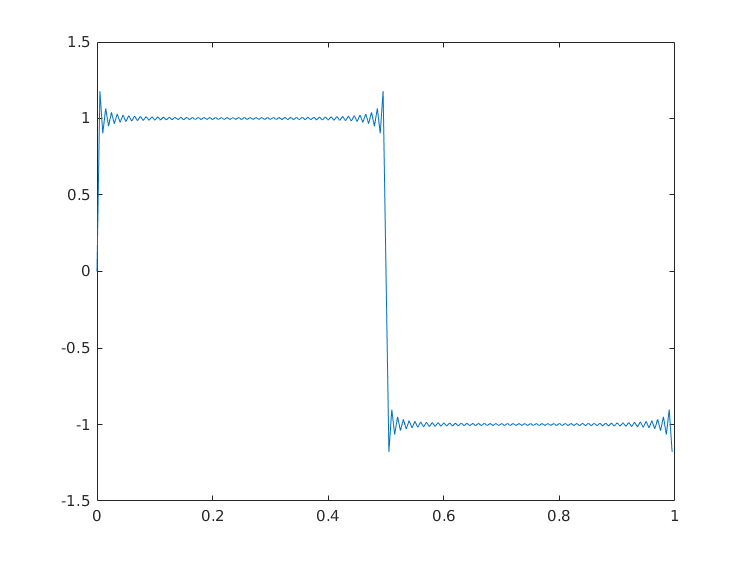
\includegraphics[scale=0.75]{figures/task1b.png}
\end{figure}

\begin{figure}
    \label{fig:task2a-bode}
    \caption{Bodediagram för G(s).}
    \centering
    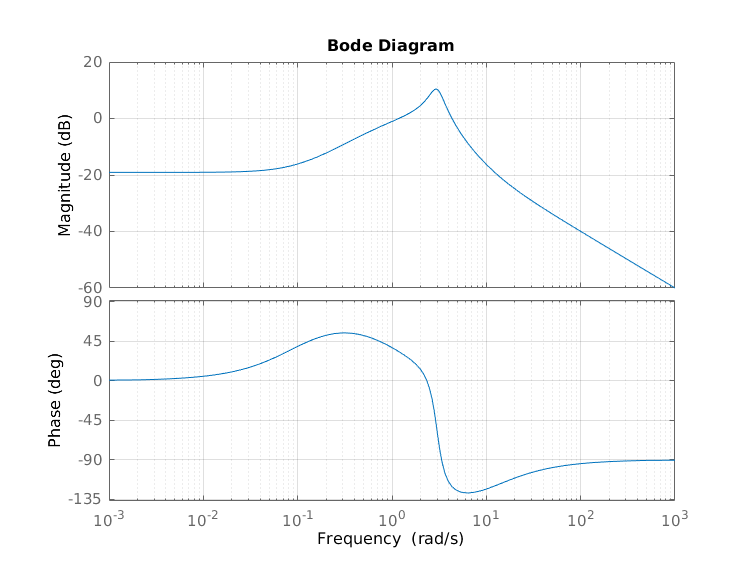
\includegraphics[scale=0.8]{figures/task2a-bode.png}
\end{figure}

\begin{figure}
    \label{fig:task2a-pzmap}
    \caption{Nod- och polgraf för G(s).}
    \centering
    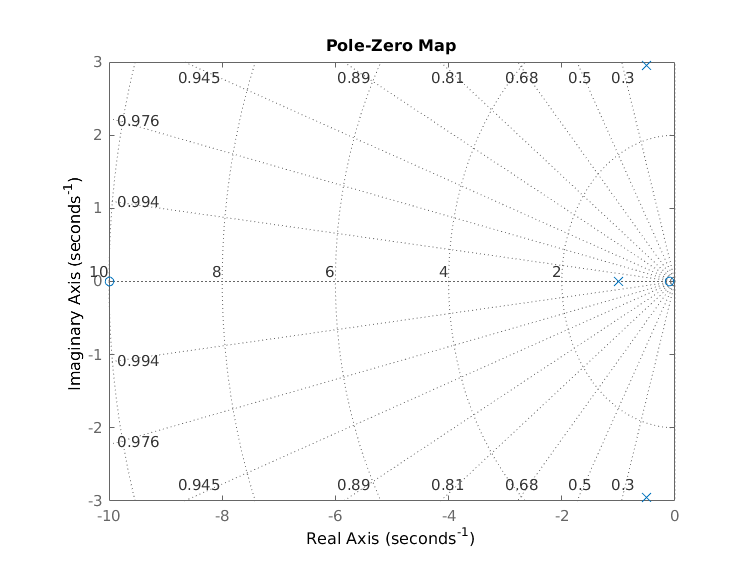
\includegraphics[scale=0.8]{figures/task2a-pzmap.png}
\end{figure}

\begin{figure}
    \label{fig:task2b}
    \caption{De tre insignalerna givna i uppgift 3.2 b).}
    \centering
    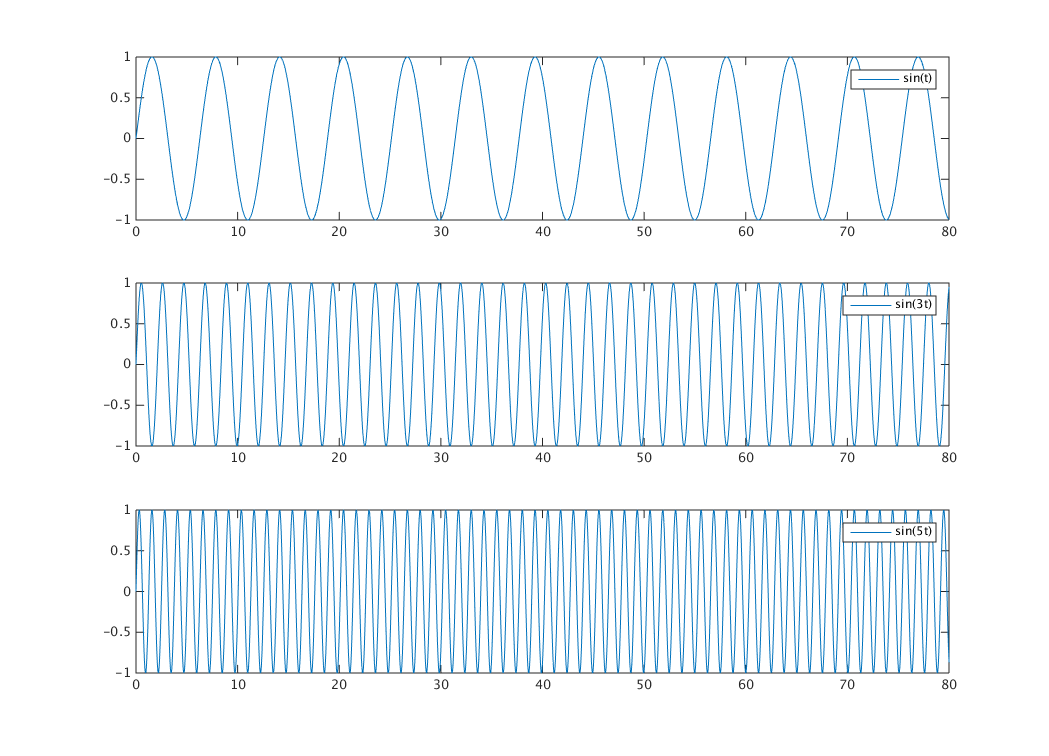
\includegraphics[scale=0.55]{figures/task2b.png}
\end{figure}

\begin{figure}
    \label{fig:task2c-three-waves}
    \caption{Utsignaler samt insignal för uppgift 3.2 c).}
    \centering
    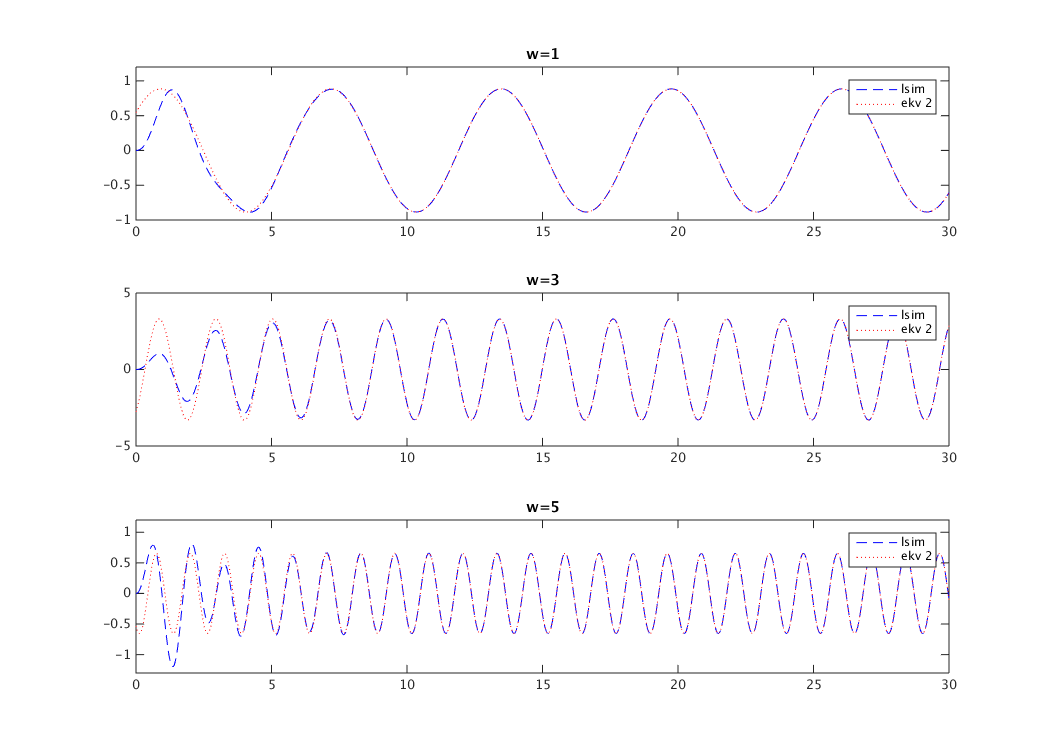
\includegraphics[scale=0.55]{figures/task2c-three-waves.png}
\end{figure}

\begin{figure}
    \label{fig:task3c-square-+-fk}
    \caption{En, av matlab genererad, fyrkantsvåg samt dess tre första -
        nollskiljda - fourierkoefficienter.}
    \centering
    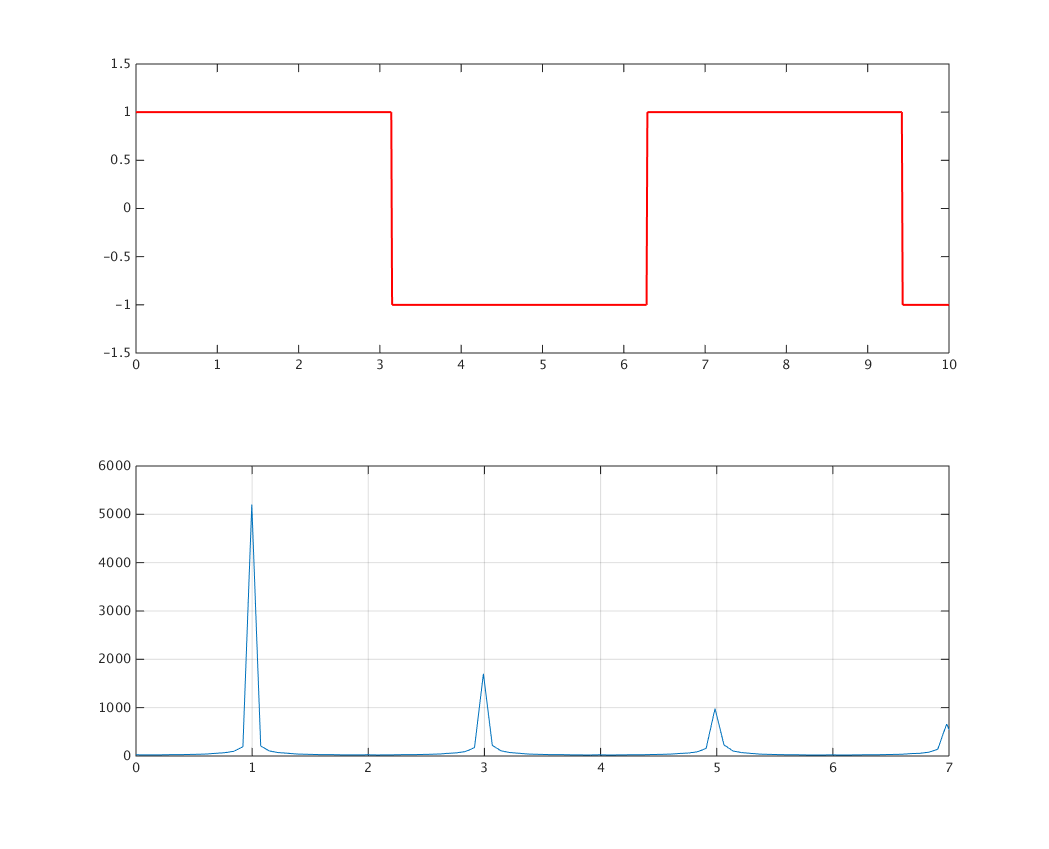
\includegraphics[scale=0.55]{figures/task3c-square-+-fk.png}
\end{figure}

\begin{figure}
    \label{fig:task3d+fk}
    \caption{De tre första - nollskiljda - fourierkoefficienterna för
    fyrkantsvågen (samma som ovan) samt för utsignalen som ges när
    fyrkantsvågen passerar systemet G(s).}
    \centering
    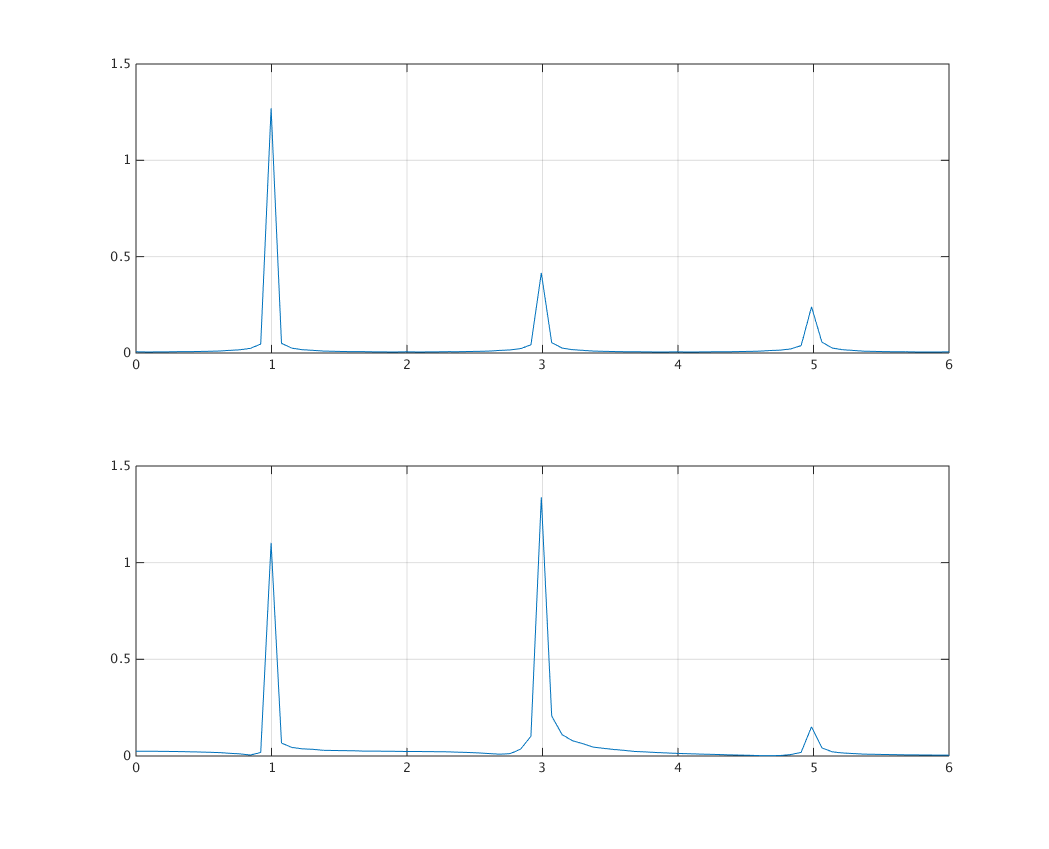
\includegraphics[scale=0.55]{figures/task3d+fk.png}
\end{figure}

\begin{figure}
    \label{fig:task4a-bode}
    \caption{Bodediagram för vårt egentillverkade system enligt uppgift 3.4 a).}
    \centering
    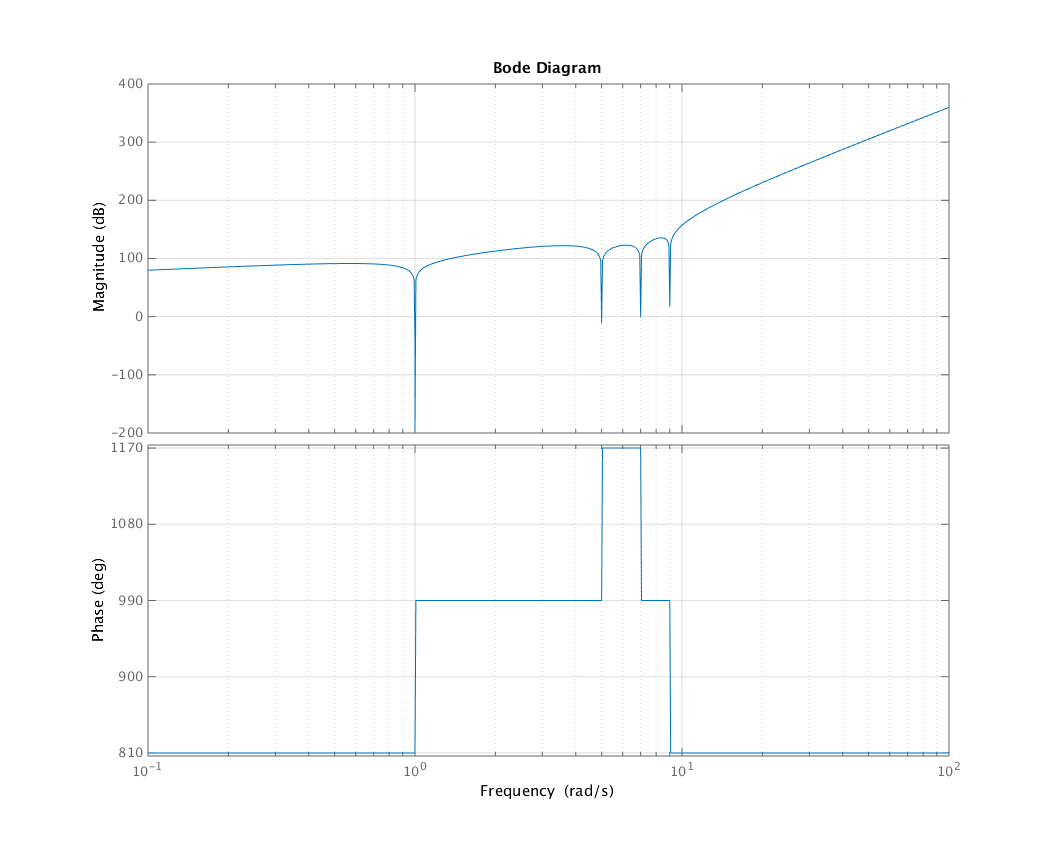
\includegraphics[scale=0.55]{figures/task4a-bode.png}
\end{figure}

\begin{figure}
    \label{fig:task4b-bode}
    \caption{Bodediagram som visar systemet efter att $\omega > 9$ dämpats.}
    \centering
    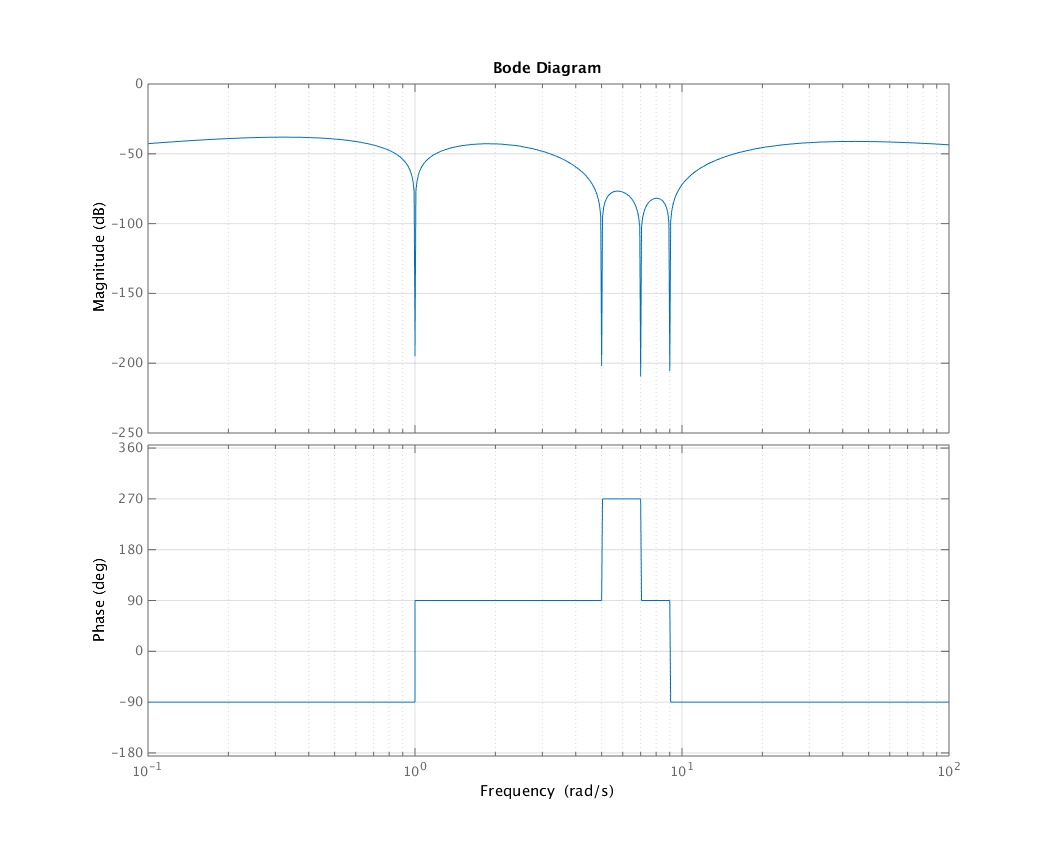
\includegraphics[scale=0.55]{figures/task4b-bode.png}
\end{figure}

\begin{figure}
    \label{fig:task4d-bode}
    \caption{Bodediagram som visar vårt system innan amplitudkorrigering i
    blått och det slutliga systemet i rött.}
    \centering
    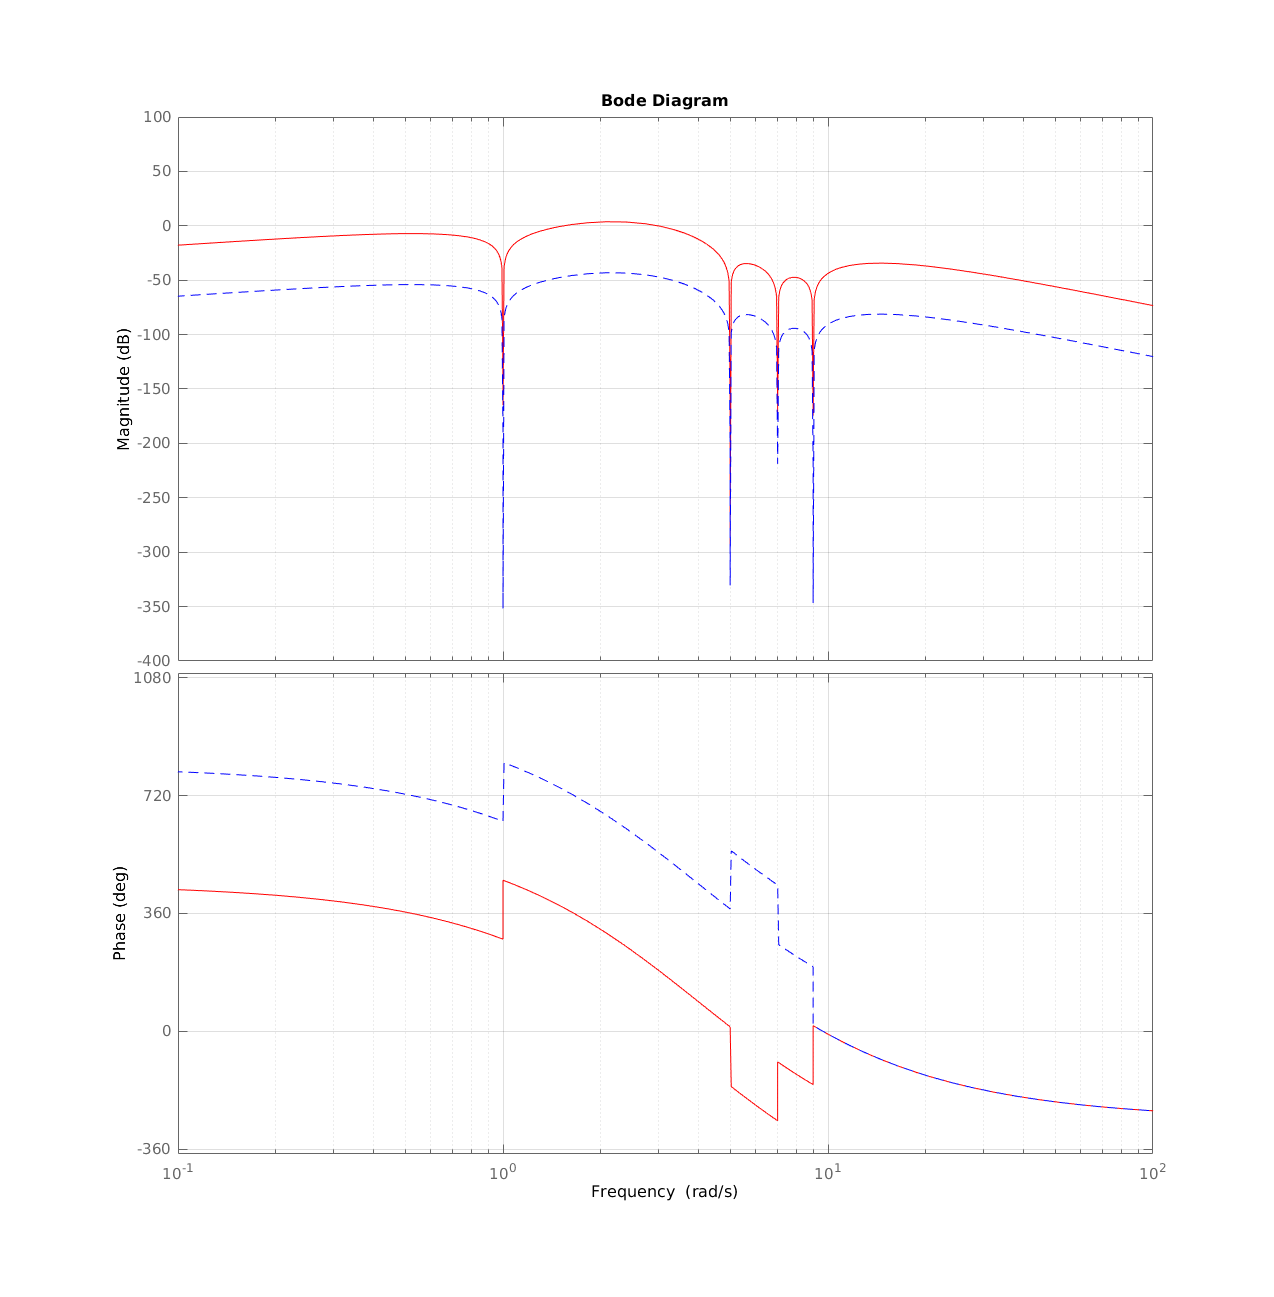
\includegraphics[scale=0.55]{figures/task4d-bode.png}
\end{figure}

\begin{figure}
    \label{fig:task4e-fk-x-sys2}
    \caption{Här ses tydligt att $\omega = 3$ släpps igenom.}
    \centering
    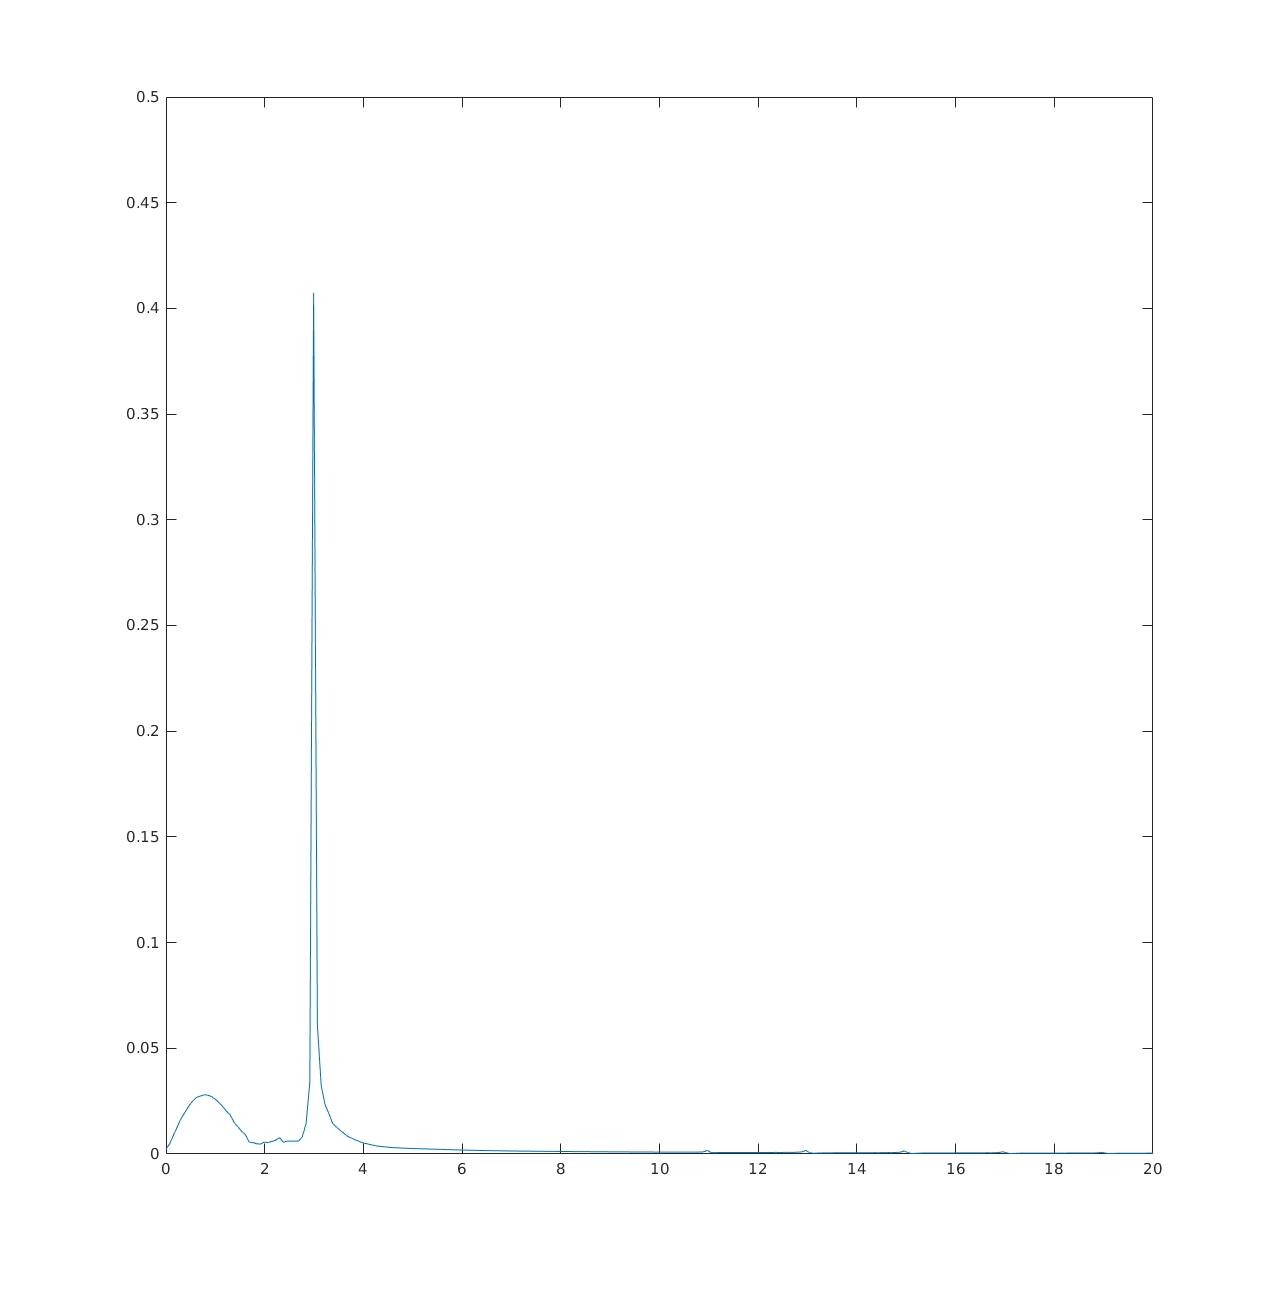
\includegraphics[scale=0.55]{figures/task4e-fk-x-sys2.png}
\end{figure}

\begin{figure}
    \label{fig:task4e-fk-y-sys2}
    \caption{Även här släpps $\omega = 3$ igenom som brukligt.}
    \centering
    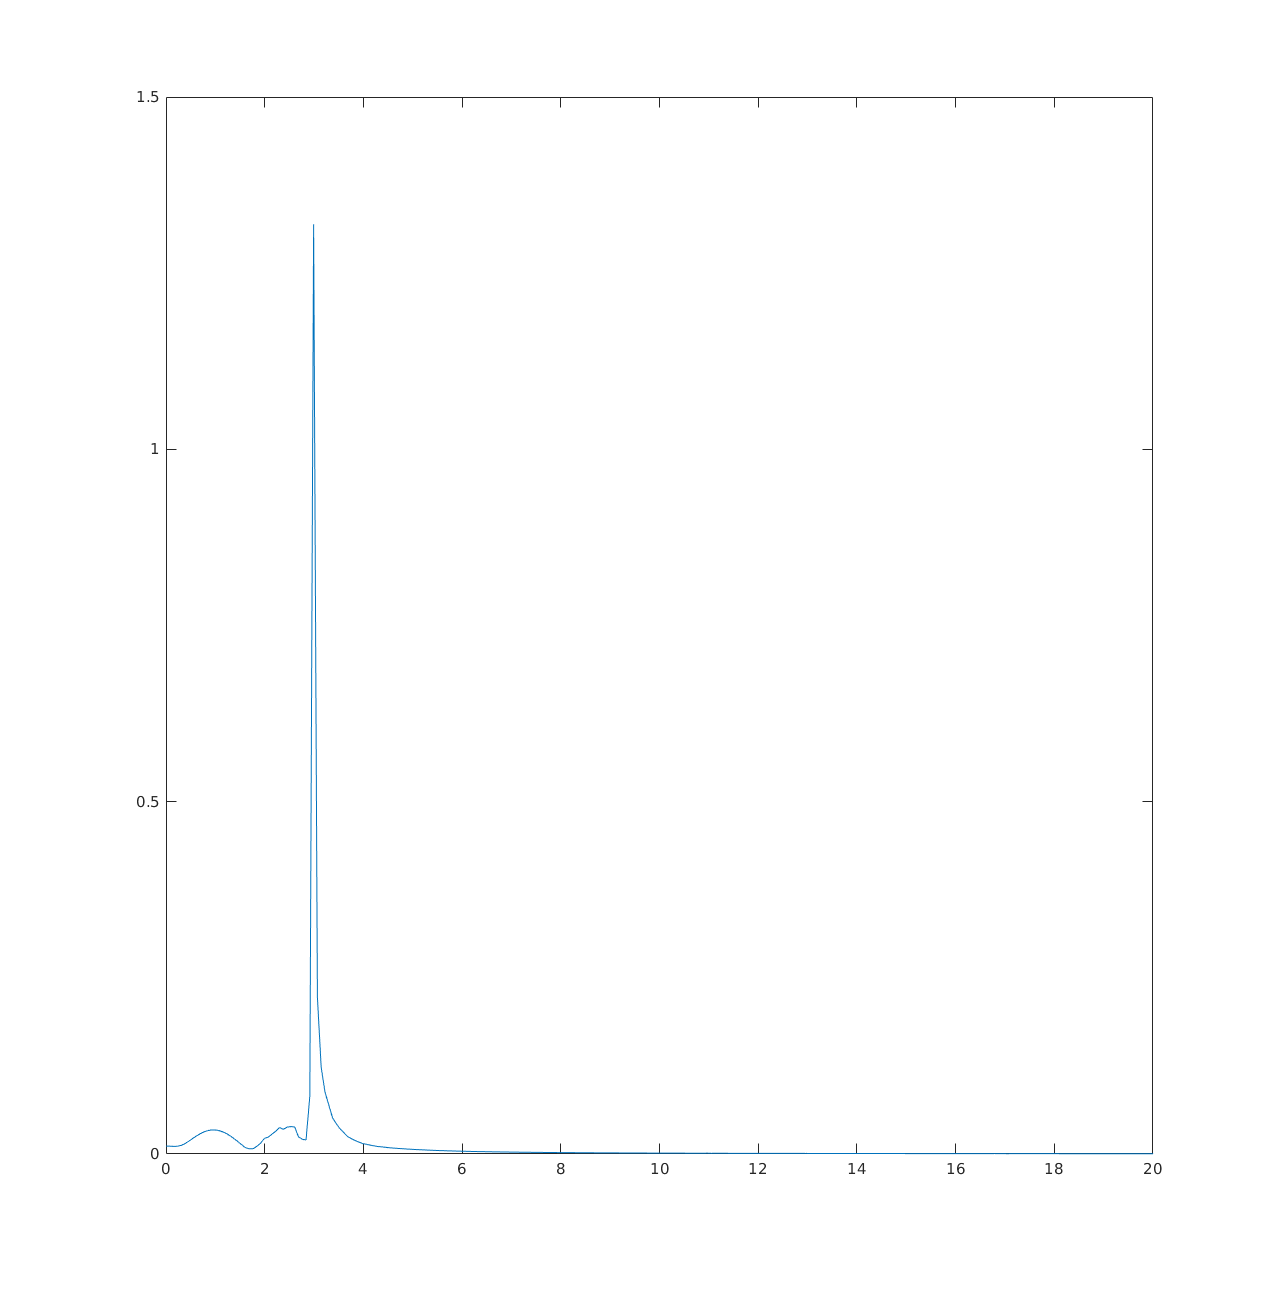
\includegraphics[scale=0.55]{figures/task4e-fk-y-sys2.png}
\end{figure}

\clearpage

\begin{figure}
    \label{fig:task4e-xsignal-sys2}
    \caption{När x-signalen passerat systemet synns tydligt att frekvensvinkeln
    $\omega = 3$ och signalen är tydligt sinusformad, om än med små
    ``skavanker''.}
    \centering
    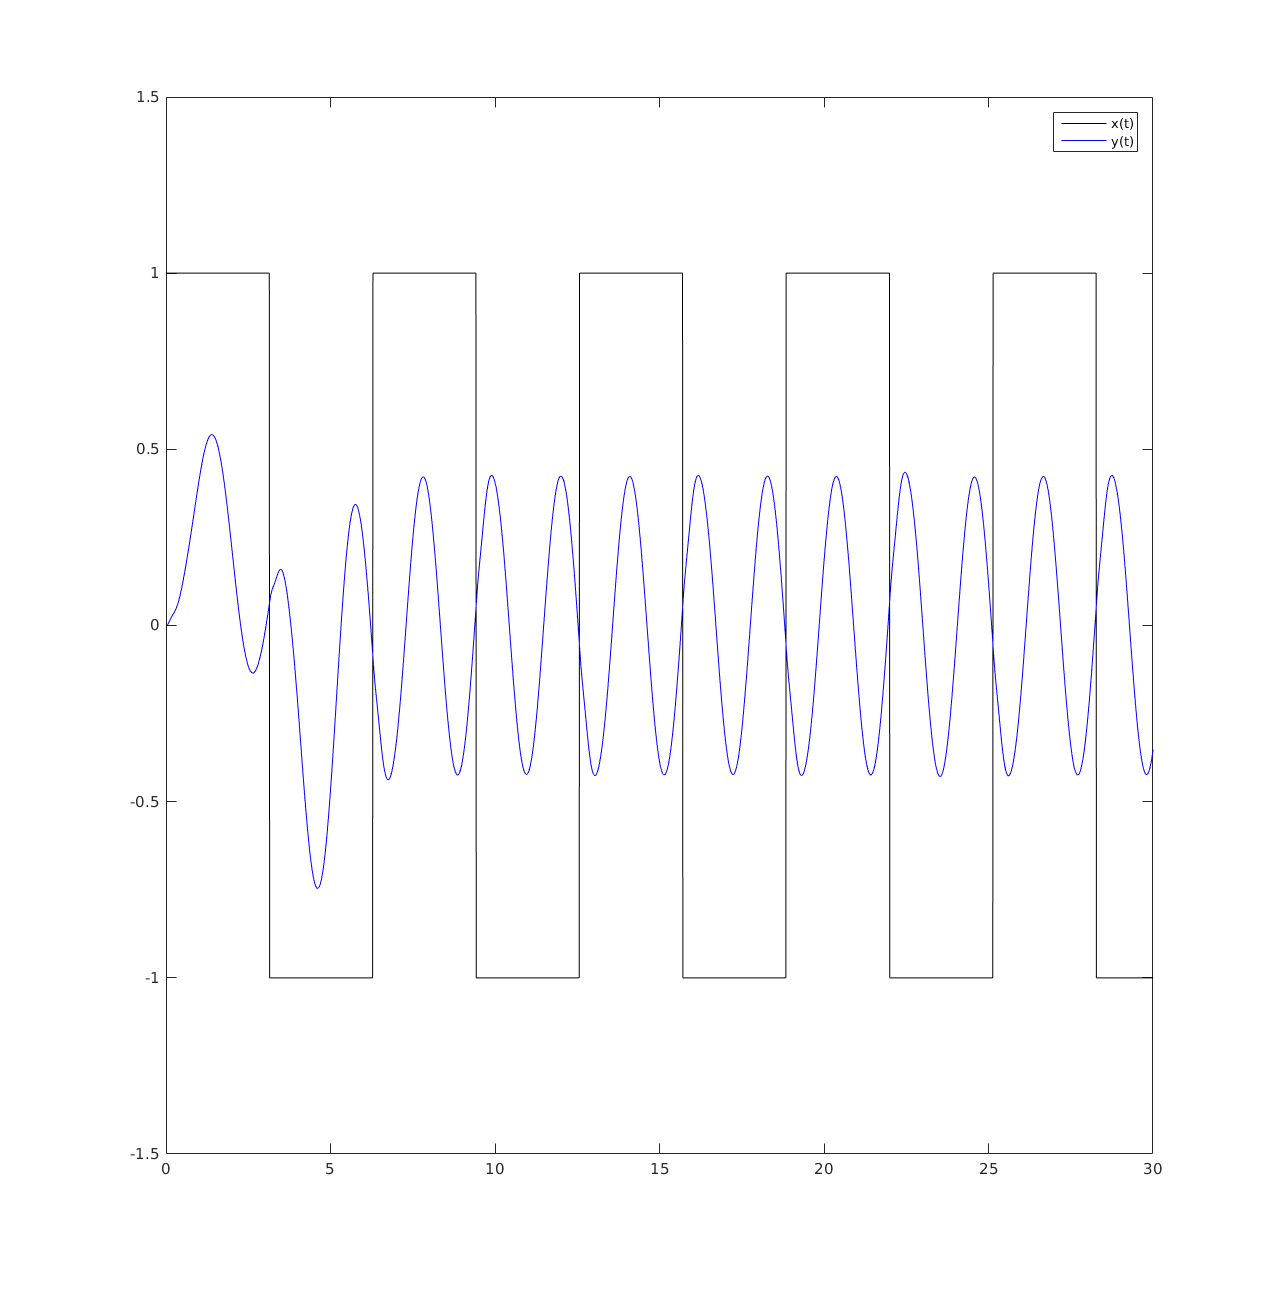
\includegraphics[scale=0.55]{figures/task4e-xsignal-sys2.png}
\end{figure}

\begin{figure}
    \label{fig:task4e-y-sys2}
    \caption{När y-signalen (fyrkantsvågen som först passerat G(s) och sedan
    vårt notchfilter) slutligen ritas upp återfinns den förväntade
    vinkelfrekvensen och sinuskarraktären.}
    \centering
    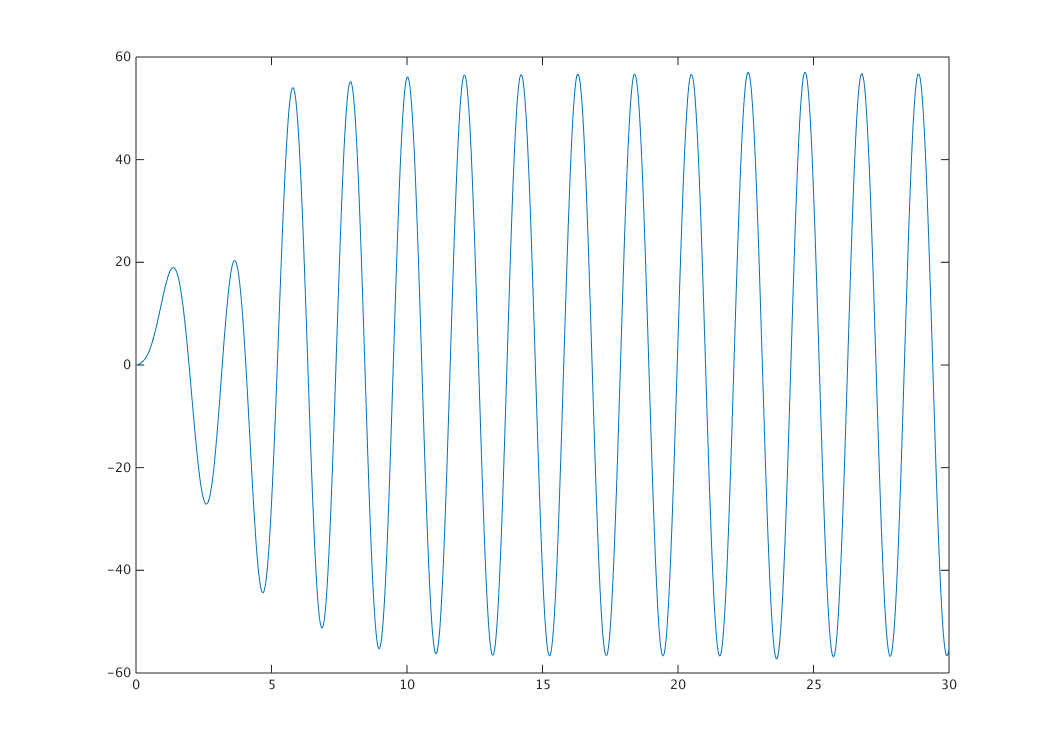
\includegraphics[scale=0.55]{figures/task4e-y-sys2.png}
\end{figure}
